\documentclass[10pt,a4paper,oneside,abstracton]{scrartcl}
\usepackage[utf8]{inputenc}
\usepackage[english, ngerman]{babel}

\usepackage{amsmath}
\usepackage{amsfonts}
\usepackage{amssymb}
\usepackage{graphicx}
\usepackage{lmodern}
	% \usepackage{kpfonts}
% \usepackage{fourier}
\usepackage[left=2cm,right=2cm,top=2cm,bottom=2cm]{geometry}
\usepackage{multicol}
\setcounter{secnumdepth}{4} %Nummerierungstiefe bis Paragraph (4. Ebene)
\usepackage{blindtext}
% \usepackage{fourier}
\usepackage[ 		%Einstellungen für Link
   colorlinks,        % Link ohne Umrandungen in zu wählender Farbe 
   linkcolor=black,   % Farbe interner Verweise 
   filecolor=black,   % Farbe externer Verweise 
   citecolor=black    % Farbe von Zitaten 
]{hyperref}

\pagestyle{empty}		%Seitenzahl wird nich angezeigt

\begin{document}

\begin{titlepage}
\par\noindent\rule{\textwidth}{0.4pt}

\noindent\begin{minipage}{0.5\textwidth}% adapt widths of minipages to your needs
		Hochschule Augsburg  \\ 
	Fakultät Elektrotechnik \\
	FB Antriebstechnik und Elektrische Maschinen
	\end{minipage}%
	\hfill%
	\begin{minipage}{0.5\textwidth}\raggedleft
		
\includegraphics[width=80pt]{./Bilder/hsLogo.jpeg}	
	\end{minipage}

	\par\noindent\rule{\textwidth}{0.4pt}
	\centering
	\vspace*{\fill}

    \vspace*{0.5cm}

    \huge\bfseries
    Elektrische Antriebe Praktikum:
	\newline 
	Bosch IndraDrive

    \vspace*{0.5cm}

    \large Jonas Hundseder, Christian Schmid
	
    \vspace*{\fill}
	\today
% \clearpage
\end{titlepage}

\tableofcontents
\clearpage


% \begin{multicols}{2}
\section{Versuchsvorbereitung}
\subsection{Massenträgheit rotatorischer Motor}
Die Schwungmasse beträgt laut Datenblatt: 
$ J_{Rot Motor} = 0,000 002 5 \frac{kg}{m^2}$. 
\newline
Die Massenträgheit der Schwungmasse wird mittels Zeichnung \ref*{Schwungmasse} berechnet.
% \begin{center}
	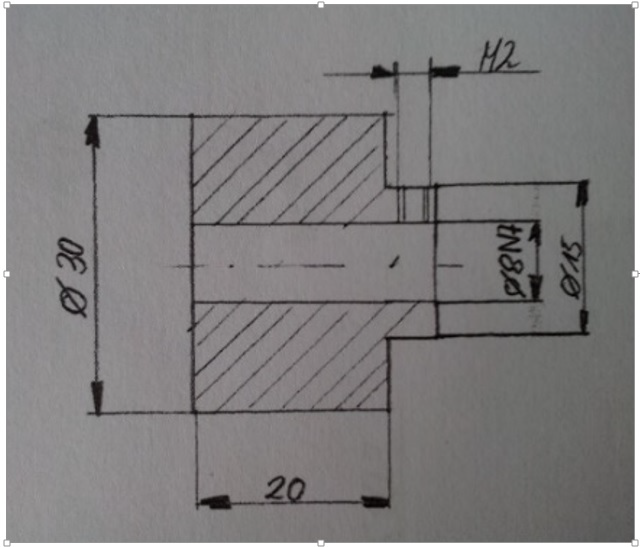
\includegraphics[width=80pt]{./Bilder/Rot_Masse.png}
\captionof{figure}[Abmaße Rotatorische Schwungmasse]{Abmaße Rotatorische Schwungmasse \label{Schwungmasse}} 
% \end{center}

Die Formel um die Massenträgheit eines Zylinders zu berechnen ist 
Formel \ref*{Formel Massentraegheit} in beschrieben: 
\begin{equation}
	J_{Zylinder} = (r_{außen}^2 - r_{innen}^2) m
	\label{Formel Massentraegheit}
\end{equation}

Die Masse des Zylinders ist nach der Formel \ref*{Formel Masse-Volumen} durch das Volumen berechenbar. 

\begin{equation}
	m = \rho V
	\label{Formel Masse-Volumen}
\end{equation}

Das Volumen eines Zylinders ist nach folgender Formel \ref*{Formel Volumen-Zylinder} berechenbar: 

\begin{equation}
	V = \pi (r_{außen}^2 - r_{innen}^2) h
	\label{Formel Volumen-Zylinder}
\end{equation}
\newline
Die Schwungmasse besteht aus Stahl. Die Dichte von Stahl beträgt: $\rho = 7,85 \cdot 10^{3}\frac{kg}{m^3}$.
\newline
Die Masse der Schwungmasse beträgt.
\newline
	$ m = 7,85 \cdot 10^{3}\frac{kg}{m^3} \cdot \pi ({15 mm}^2 - {4 mm}^2) 20 mm = 0,103 kg$
\newline
	Die Massenträgheit der Schwungmasse beträgt: 
	\newline
	$ J_{Schwungmasse} = ({15 mm}^2 - {4 mm}^2) \cdot 0,103 kg = 21,54 \cdot 10^{-6} \frac{kg}{m^2}$
	Die gesamte Massenträgheit beträgt 
	\newline
	$J_{Gesamt} =  J_{Schwungmasse}+ J_{Motor} = 21,54 \cdot 10^{-6} \frac{kg}{m^2} + 2,5 \cdot 10^{-6} \frac{kg}{m^2}= 21,54 \cdot 10^{-6} \frac{kg}{m^2}$
	\newline
	\newline
	\subsection{Verschiebezeit Linearmotor}
	Die minimale Verschiebezeit um die maximale Strecke des Linearmoduls zu verfahren wird berechnet. 
	\newline
	Die Gleichungen \ref*{Formel Beschleunigung} und \ref*{Formel Weg} sind die Grundgleichungen aus der Kinematik und werden benötigt:

\begin{equation}
	a = \frac{\Delta v}{\Delta t}
	\label{Formel Beschleunigung}
\end{equation}

\begin{equation}
	s_{Ges} =  \frac{1}{2} a t^2 + v t +S_0
	\label{Formel Weg}
\end{equation}
Die Hochlaufzeit und die Abbremszeit sind identisch. 
\newline 
Die maximale Beschleunigung ist gleich der maximalen Verzögerung. 
Daher gilt die Formel \ref*{Formel TAbbrems}. 
\newline 
\begin{equation}
	t_{Hochlauf} = \frac{\Delta v}{a} = t_{Abbrems}
	\label{Formel TAbbrems}
\end{equation}
In unserem Fall lautet die Formel für den Weg:
\begin{equation}
	s_{Ges} =  \frac{1}{2} a t^2_{Hochlauf} + v_{Max} t_{Konstant} + \frac{1}{2} a t^2_{Abbrems} 
	\label{Formel Weg Beispiel}
\end{equation}
Die Problemstellung sieht schmetisch wie folgt aus. 
Die Geschwindigkeit ist das Integral der Beschleunigung $ v = $\(\int_{a}^{b} a \,dt\). Die Geschwindigkeit steigt und fällt bei konstanter Beschleunigung linear. 
\newline

\begin{figure}
\begin{center}
	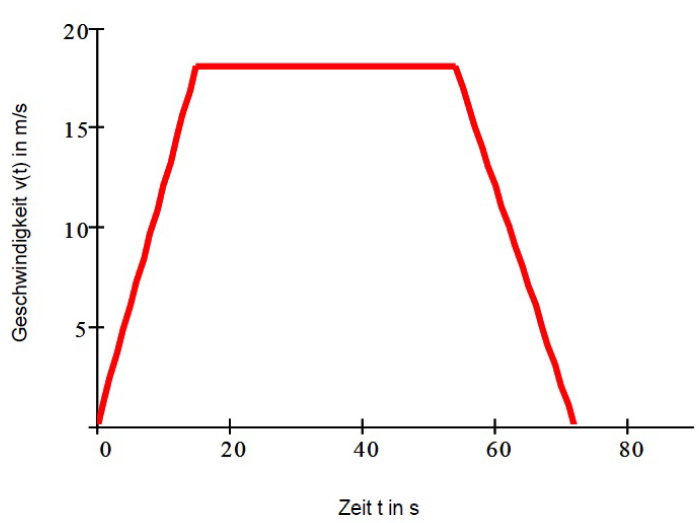
\includegraphics[width=200pt]{./Bilder/Geschwindigkeit.png}
	\captionof{figure}[Beschleunigung und Verzögerung im v/t Diagramm]{Beschleunigung und Verzögerung im v/t Diagramm \label{v/t Diagramm}} 
	\cite{Uebung1}
	% \captionsource{Caption}{Antriebstechnik Übung 1}
\end{center}
\end{figure}
Der Weg ist das Integral der Geschwindigkeit $ s = $\(\int_{a}^{b} v \,dt\). Bei linearem Geschwindigkeitsanstieg steigt der Weg quadratisch. 
Bei konstanter Geschwindigkeit steigt der Weg linear an. 
\begin{figure}
	\begin{center}
		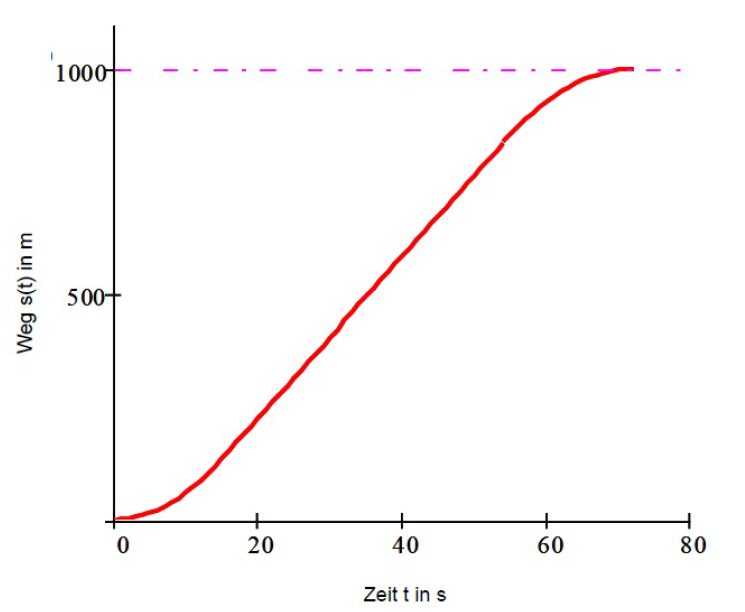
\includegraphics[width=200pt]{./Bilder/weg.png}
		\captionof{figure}[Beschleunigung und Verzögerung im s/t Diagramm]{Beschleunigung und Verzögerung im s/t Diagramm \label{s/t Diagramm} }
		\cite{Uebung1}
	\end{center}

\end{figure}


Wird die Formel \ref*{Formel Weg Beispiel} nach $t_{Konstant} $ umgestellt ergibt sich Formel \ref*{Formel t Konstant}.

\begin{equation}
	t_{Konstant} = \frac{s_{Ges} - a t^2_{Hochlauf}}{v_{Max}} =
	 \frac{s_{Ges}}{v_{Max}} - \frac{v_{Max}}{a_{Max}}
	\label{Formel t Konstant}
\end{equation}
Die Formel für die gesamte Zeit lautet: 
\begin{equation}
	t_{Gesamt} = t_{Konstant} + t_{Hochlauf} + t_{Abbrems} 
\end{equation}
\newline
Die Hochlaufzeit $t_{Hochlauf} $ beträgt: 
\begin{equation}
	t_{Hochlauf} = \frac{\Delta v_{Max}}{a_{Max}} = \frac{0,2 \frac{m}{s} }{48,4 \frac{m}{s^2} } = 4,13 \cdot 10^{-3}s
\end{equation}
Die Zeit mit maximaler Geschwindigkeit beträgt: 
\begin{equation}
t_{Konstant} = \frac{s_{Ges}}{v_{Max}} - \frac{v_{Max}}{a_{Max}} = 
\frac{70 \cdot 10^{-3} m} {0,2 \frac{m}{s} } 
- \frac{0,2 \frac{m}{s}}{48,8 \frac{m}{s^2}} = 0,345 s
\end{equation}
Die gesamte Verschiebezeit beträgt: 
\begin{equation}
	t_{Gesamt} = t_{Konstant} + t_{Hochlauf} + t_{Abbrems} = 0,345,87 s + 4,13 \cdot 10^{-3} s \cdot 2 = 0,354 s
\end{equation}
\section{Feedback zum Versuch}

\newpage

\listoffigures


\begin{thebibliography}{9}

\bibitem{Uebung1}
	Prof. Dr. Meyer	Vorlesung Antriebstechnik Übung 1

\end{thebibliography}

% \end{multicols}
 

\end{document}
